\section{Related Work}\label{sec:related_work}

\subsection{Lighting Representations} 

\begin{figure*}
    \centering
    \makebox[\textwidth]{%
        \begin{tikzpicture}
    
        \node (img) {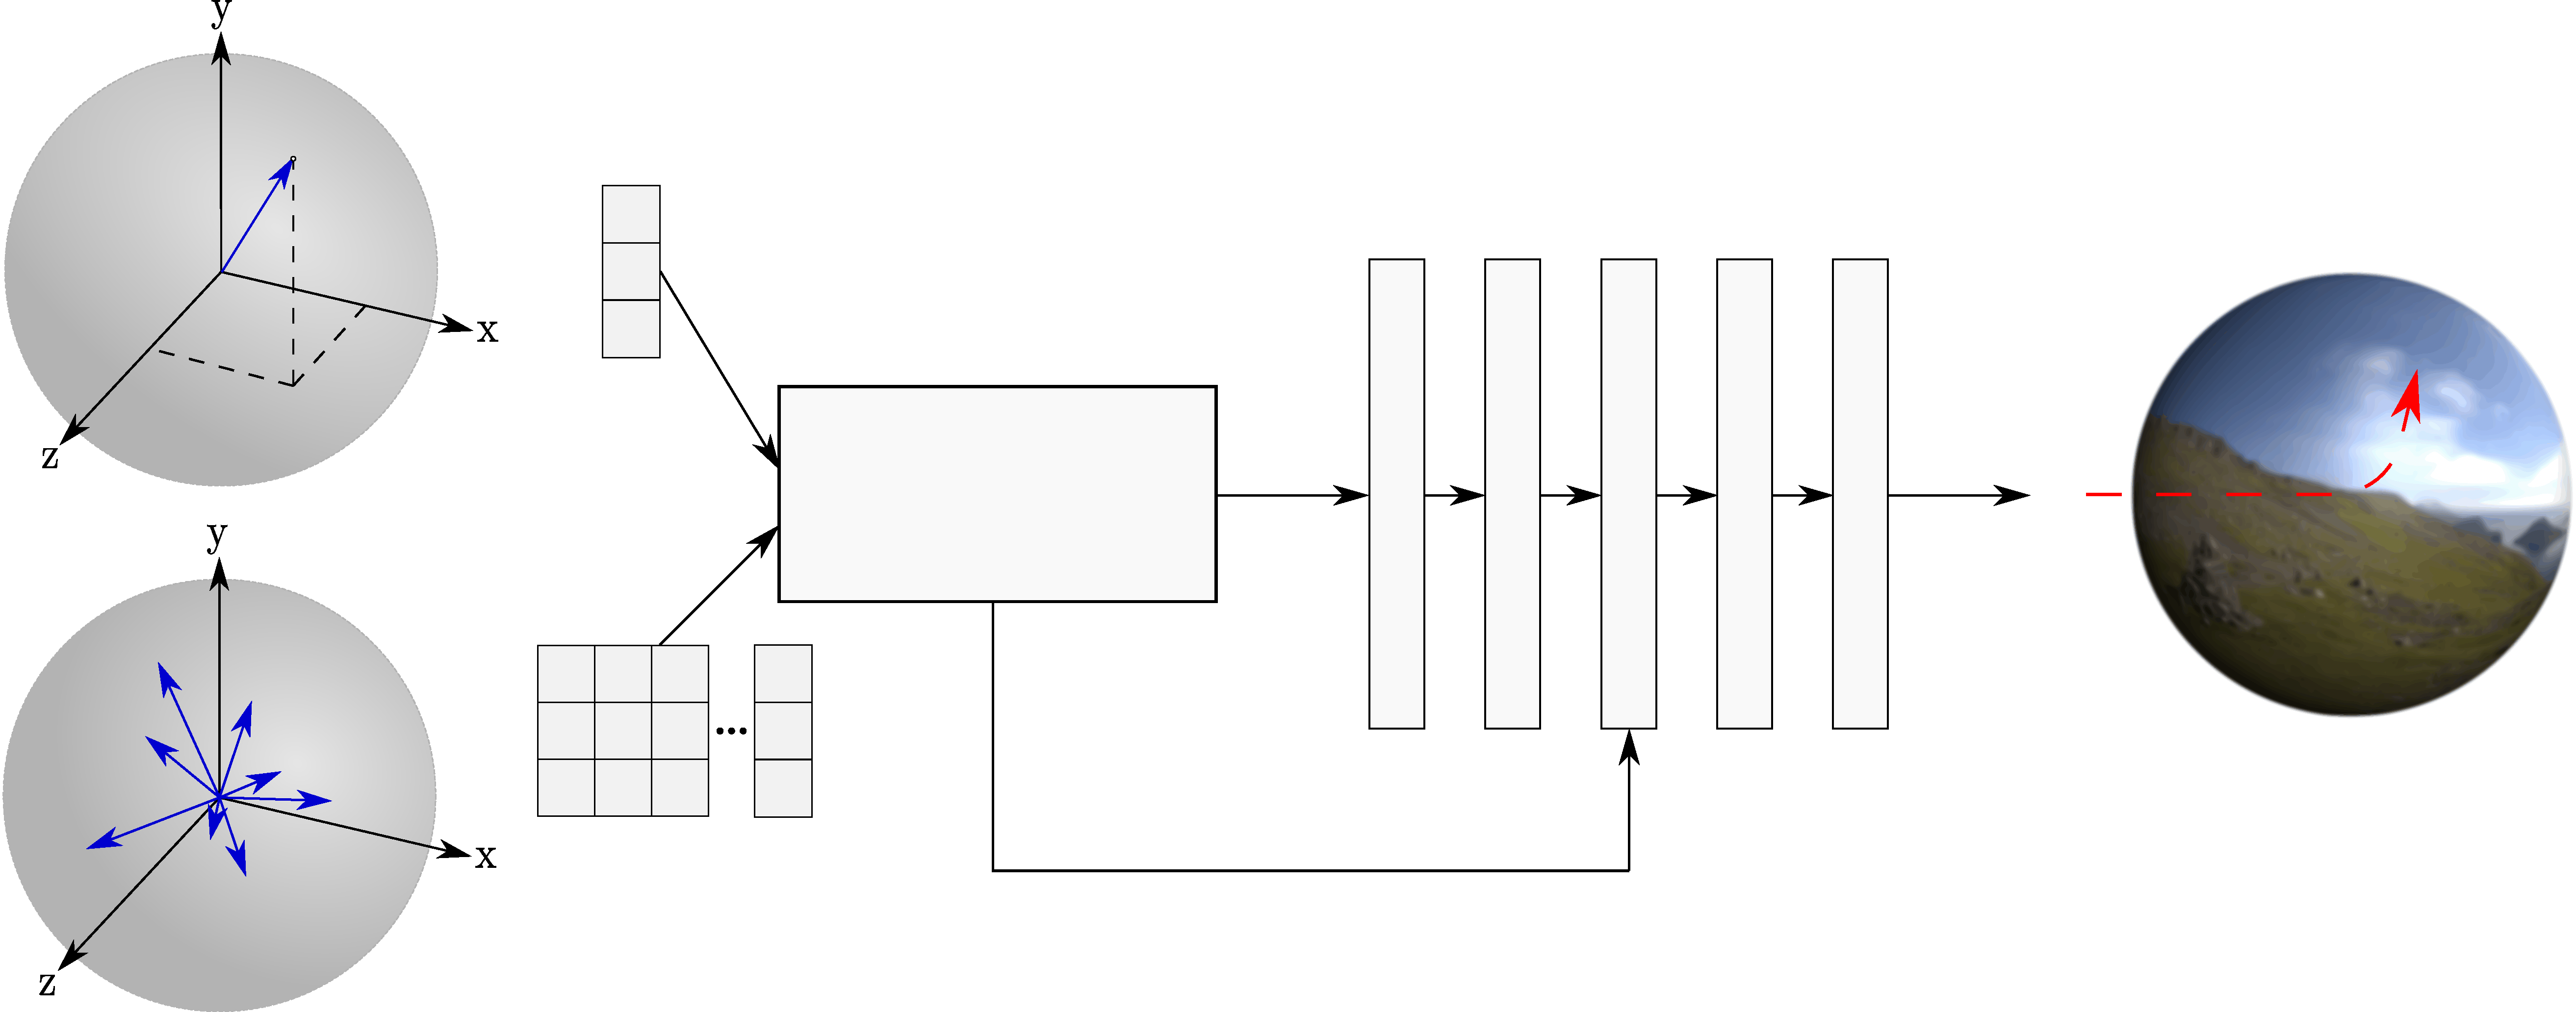
\includegraphics[width=0.98\textwidth]{Figures/conditional_spherical_neural_fields.pdf}};
        \node at (-4.56,2.04) {$x$};
        \node at (-4.56,1.63) {$y$};
        \node at (-4.56,1.24) {$z$};
        \node at (-4.25,-2.5) {$3 \times N$};
        \node at (-6.7,2.5) {$\mathbf{d}$};
        \node at (-6.7,-1.5) {$\mathbf{Z}$};
        \node at (0.0,-0.2) {$\mathbf{d}^\prime$};
        \node at (0.25,-2.2) {$\mathbf{Z}^\prime$};
        \node at (5.3, 0.08) {$\mathbf{C}$};
        \node at (2.35,2.5) {Rotation-Equivariant Conditional};
        \node at (2.35,2.1){Spherical Neural Field};
        \node at (-2.0,0.3){Invariant}; 
        \node at (-2.0,-0.1){Transformation};
        \node at (-8.5,2.9) [rotate=45] {\small Query};
        \node at (-8.5,-0.7) [rotate=45] {\small Latent Code};
        \end{tikzpicture}
    }
    \caption{We propose to represent a space of spherical signals via a rotation-equivariant conditional spherical neural field. The signal in a direction $\mathbf{d}$ can be queried by evaluation of the network and rotating the Vector Neuron conditioning latent code $\mathbf{Z}$, corresponds to rotating the spherical signal.}
\end{figure*}

An illumination environment is a spherical signal. A relatively small set of alternatives are used for their representation within vision and graphics. A widely used representation in graphics is an environment map \cite{ramamoorthi_frequency_2002, ramamoorthi_efficient_2001, tsai_all-frequency_2006, wang_all-frequency_2009}, which is a regularly sampled 2D image representing a flattening of the sphere, usually via an equirectangular projection. However, the projection introduces distortions leading to irregular sampling on the sphere, it is not compact, introduces boundaries and provides no prior for inverse problems. Nevertheless, environment map representations have been used in inverse settings where every pixel in the map is optimised independently \cite{sengupta_neural_2019}.

Spherical harmonic (SH) lighting \cite{basri_lambertian_2003,ramamoorthi_efficient_2001} is a compact lighting representation commonly used in real-time computer graphics \cite{ramamoorthi_efficient_2001, green_spherical_2003, sloan_precomputed_2002} and inverse rendering \cite{yu_outdoor_2021, tsai_all-frequency_2006, li_inverse_2020, rudnev_nerf_2022, egger_occlusion-aware_2018}. While SHs can be used to represent the illumination environment directly, more commonly, they represent pre-integrated lighting, i.e.~the illumination environment convolved with a bidirectional reflectance distribution function (BRDF). When the BRDF is low frequency, as it is for Lambertian reflectance, then the convolution is also low frequency making the SH approximation very accurate \cite{basri_lambertian_2003}. 

An alternative, growing in popularity, is the Spherical Gaussian (SG) representation \cite{wang_all-frequency_2009, tsai_all-frequency_2006, zhang_physg_2021}. SGs represent a lighting environment as a collection of Gaussian lobes on the sphere, each of which has 6 degrees of freedom (three for RGB amplitude, two for spherical direction and one for sharpness). While this allows the reconstruction of localised high-frequency features, it still requires many lobes to approximate complex illumination environments. Li et al.~\cite{li_inverse_2020} compare SH and SG for object re-lighting, finding SG was able to recover higher frequency lighting using a similar number of parameters as SH, though both still required a large number of parameters to approximate ground truth. SGs are now widely used in inverse rendering \cite{zhang2021physg}.

Both SHs and SGs are \emph{rotation equivariant}. A rotation of the illumination environment corresponds directly to a rotation of the SH basis or the SG lobe directions. Equivalently, they can represent any rotation of a given environment with equal accuracy. However, they provide no prior over the space of possible illuminations. SGs or SHs can represent any colour of light coming from any direction.

\subsection{Illumination Priors} 

While it has long been known that natural illumination environments exhibit statistical regularities \cite{dror_statistical_2004}, this has largely been overlooked in prior work. Here we describe the small number of exceptions. Barron and Malik \cite{barron2014shape}, Egger et al.~\cite{egger_occlusion-aware_2018}, and Yu and Smith \cite{yu_outdoor_2021} learn a linear statistical model with Gaussian prior in the space of SH coefficients. Both Barron and Malik \cite{barron2014shape} and Yu and Smith \cite{yu_outdoor_2021} learn their model from a curated set of known environments maps, while Egger et al.~\cite{egger_occlusion-aware_2018} use indirectly observed illumination environments estimated from fitting a morphable model to face images. Barron and Malik \cite{barron2014shape} build their model in log space as they found the Gaussian assumption on SH parameters to hold better. While providing a useful constraint to avoid unrealistic illumination environments, these approaches inherit the weakness of SHs in being unable to reproduce high-frequency lighting effects while also losing the rotation equivariance. Yu and Smith \cite{yu_outdoor_2021} seek to overcome this by rotation augmentation at training time, but this brute force approach makes no guarantee of rotation equivariance. The same illumination model was later used in an inverse rendering setting that also estimated cast shadow maps \cite{yu2022outdoor} but these were unconstrained and not related to geometry or occlusion testing of the illumination environment.

Sztrajman et al.~\cite{sztrajman_high-dynamic-range_2020} separate environment maps into HDR and LDR components. Using a CNN-based auto-encoder for estimations of LDR components of lighting alongside a low dimensional SG model for the HDR lighting provided by the sun. They too require data augmentation in the form of rotations, can make no equivariance guarantees and, due to the low dimensionality of the SG model, struggle to represent environments with multiple HDR light sources.

Several other neural-based HDR environment map models have followed since RENI. Both Somanath et al.~\cite{Somanath_2021_CVPR} and Dastjerdi et al.~\cite{dastjerdiEverLightIndoorOutdoorEditable2023} learn to predict a full HDR environment map from a narrow field-of-view LDR camera image. Unlike our work, Somanath et al.~\cite{Somanath_2021_CVPR} do not learn a prior and cannot sample from their latent space. Dastjerdi et al.~\cite{dastjerdiEverLightIndoorOutdoorEditable2023} allows parametric control over the lighting direction a Spherical Gaussian representation of the dominant light source. Chen at el.~\cite{chenText2LightZeroShotTextDriven2022} learn a text-to-HDR environment map model via a CLIP \cite{radfordLearningTransferableVisual2021} conditioned global code-book sampler and a structure-aware local code-book sampler. They propose a novel Super-Resolution Inverse Tone Mapping Operator (SR-iTMO) to simultaneously increase the spatial resolution
and dynamic range of the environment map. Yao et al.~\cite{yaoNeILFNeuralIncident2022} model incident light at a point for a given direction as a 5D light field network allowing the modelling of spatially varying illumination effects. Lyu et al.~\cite{lyuDiffusionPosteriorIllumination2023a} train an unconditional diffusion model \cite{hoDenoisingDiffusionProbabilistic2020} to generate realistic environment maps. Then, in an inverse rendering setting, gradients from a differentiable path tracer are used to update the posterior score function such that the diffusion model generates an environment map to explain the image. Hold-Geoffroy et al.~\cite{Hold-Geoffroy_2019_CVPR} learn a sky-model through autoencoding HDR sky panoramas and apply this in an image to sky-estimation task. It is trained on the Laval HDR sky database and the SUN360 HDR database. The model however does segment the sky explicitly and only models sky and not the full environment. It does not tackle the challenge of rotation equivariance and, since it is CNN-based, is restricted to directions on the original grid. Our neural field formulation means we can evaluate illumination in any direction.

A separate body of works derives physical models of sky illumination. For example, modelling the total luminance arriving at a point on Earth \cite{PEREZ1993235}. Such models capture only the light arriving from the upper (sky) hemisphere, for example for the purpose of rendering Earth as viewed from space \cite{10.1145/166117.166140}. Such models \cite{10.1145/311535.311545,10.1145/2185520.2185591} do not provide a \emph{prior}, i.e.~a learnt low dimensional statistical model of the likelihood of different incident illumination fields. Mirbauer et al.~\cite{mirbauer2024skygan} proposed a hybrid approach that used an analytical model for sunlight which conditioned a GAN that generates cloudy skies. Satilmis et al.~\cite{satilmis2022deep} take a similar approach but use artist drawn cloud maps to condition generation. Such sky illumination models have been used in the context of inverse rendering \cite{yu2021hierarchical,zhu2021spatially}. However, all of these approaches do not model occlusion of the upper hemisphere by the horizon (for example due to trees and buildings) or second bounce light from the ground. This is captured in our model by learning a full spherical representation. 

\subsection{Neural Fields}

Neural fields \cite{xie_neural_2021} have provided impressive results in a range of applications including representations of objects and scenes \cite{sitzmann_implicit_2020, atzmon_sal_2020, mescheder_occupancy_2019, chibane_neural_2020, chen_learning_2019, gropp_implicit_2020, park_deepsdf_2019, tancik_block-nerf_2022}, in inverse rendering \cite{boss_nerd_2021, bi_neural_2020, rudnev_nerf_2022, srinivasan_nerv_2020, boss_neural-pil_2021, zhang_physg_2021} and robotics \cite{li_3d_2021, chen_full-body_2021, ortiz_isdf_2022}. The work most closely related to ours is Neural-PIL \cite{boss_neural-pil_2021}. They use a FiLM SIREN similar to that proposed in Pi-GAN \cite{chan_pi-gan_2021}, and like us use a direction query vector and auto-decoder architecture. However, they do not have rotation-equivariance and apply no natural light prior. They also model pre-integrated lighting, conditioning the latter layers of their FiLM SIREN on a material roughness parameter. \cite{rebainAttentionBeatsConcatenation2023} evaluated the effectiveness of three possible conditioning methods for neural fields and found that attention-based conditioning was the most effective. In RENI++ we too found that a transformer-based architecture outperformed both a conditioned-via-concatenation and FiLM conditioned SIREN.

\subsection{Invariance and Equivariance}\label{sec:litrevinv}

Two important symmetries in computer vision are invariance and equivariance to the rotation group \cite{bronstein_geometric_2021}. Some works attempt to achieve these properties via data augmentation \cite{yu_outdoor_2021, qi_pointnet_2017, sztrajman_high-dynamic-range_2020}, which still results in missed cases for continuous rotations. A solution alleviating the need for extensive data augmentation is the Vector Neuron \cite{deng_vector_2021}, which offers a framework for designing $SO(3)$-equivariant or invariant networks via a latent matrix representation rather than a latent vector. They propose extensions of classical scalar neuron layers to vector neuron layers that are equivariant or invariant to rotations of their input latent matrix representation. The design of these layers hinges on the orthogonality of rotation matrices. We therefore note that vector neuron layers are in fact $O(3)$-equivariant or invariant, since the more general orthogonal group also satisfies the orthogonality property. This means that vector neuron networks are equivariant or invariant to reflections as well as rotations. Vector Neurons were originally designed for rotation equivariant or invariant processing of point cloud data. We re-purpose them for the representation of spherical signals such as environment maps. Other works have also incorporated rotation equivariance into their latent representation. For example, HoloGAN \cite{nguyen2019hologan} uses a volumetric 3D latent space, a rotation of which corresponds to a 3D rotation of the modelled object. However, decoding their latent space amounts to volume rendering the latent space to produce a perspective 2D image whereas our rotation equivariant latent space directly conditions a spherical neural field.

Another commonly sought invariance is to scale. For example, in the monocular depth estimation problem, absolute depth is often unobtainable due to a lack of calibration information. For this reason, scale-invariant losses \cite{eigenDepthMapPrediction2014} are often used, such that the depth prediction network learns to estimate only relative scale. The output depth map is then only valid up to an unknown scale. We take the same approach in learning a model of natural illumination. An environment map is a representation of a real environment but at arbitrary scale (dependent on camera exposure and the subsequent image processing pipeline). Our model therefore learns the relative brightness of natural environments and the absolute scale becomes an additional optimsable parameter when fitting to data.